\begin{figure}[h]
    \centering
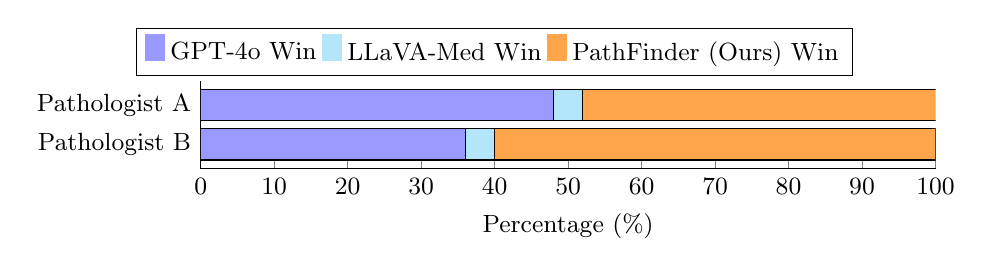
\begin{tikzpicture}
    \begin{axis}[
        width=0.9\linewidth,
        height=2.7cm,
        xbar stacked,
        bar width=0.4cm, % height, because we flipped.
        xmin=0, xmax=100,
        axis x line*=bottom,
        axis y line*=left,
        ymin=-0.2, ymax=1.2, % add some buffer border
        ytick=data,
        yticklabels={Pathologist B, Pathologist A},
        % nodes near coords,
        % nodes near coords align={left},
        enlarge y limits=0.3,
        xlabel={Percentage (\%)},
        % legend style={font=\small, at={(0.4,1.6)}, anchor=north, legend columns=-1},
        tick label style={font=\small}, % Adjust tick labels
        label style={font=\small},      % Adjust axis labels
        legend style={font=\small, at={(0.4,1.6)}, anchor=north, legend columns=-1},
        legend image code/.code={
            \draw[#1, draw=none] (0cm,-0.1cm) rectangle (0.25cm,0.25cm);
        },
    ]
    % A's score label and bars
    \addplot[fill=blue!40] coordinates {(36,0) (48,1)}
        node[anchor=east, xshift=-1em] at (axis cs:0,0) {Pathologist A's score};  % Label for A's score at (36,0)
    
    % B's score label and bars
    \addplot[fill=cyan!30] coordinates {(4.0,0) (4.0,1)}
        node[anchor=east, xshift=-1em] at (axis cs:0,1) {Pathologist B's score};  % Label for B's score at (4,0)
    
    % Additional bars without labels
    \addplot[fill=orange!70] coordinates {(60,0) (48.1,1)};
    
    \legend{GPT-4o Win, LLaVA-Med Win, PathFinder (Ours) Win}
    \end{axis}
\end{tikzpicture}

\caption{Expert human pathologist preferences for each model in assessing description quality, evaluated in a double-blind survey for unbiased comparison.}

\label{fig:pathologist-analysis}
\end{figure}